%% BioMed_Central_Tex_Template_v1.06

%%% additional documentclass options:
%  [doublespacing]
%  [linenumbers]   - put the line numbers on margins

%%% loading packages, author definitions

%\documentclass[twocolumn]{bmcart}% uncomment this for twocolumn layout and comment line below
\documentclass{configs/bmcart}

%%% Load packages
%\usepackage{amsthm,amsmath}
%\RequirePackage{natbib}
%\RequirePackage[authoryear]{natbib}% uncomment this for author-year bibliography
%\RequirePackage{hyperref}
%\usepackage[utf8]{inputenc} %unicode support
%\usepackage[applemac]{inputenc} %applemac support if unicode package fails
%\usepackage[latin1]{inputenc} %UNIX support if unicode package fails
\usepackage{graphicx}
\usepackage{url}
\usepackage[acronym]{glossaries}

\makeglossaries
\newacronym{roi}{ROI}{region of interest}
\newacronym{sfm}{SfM-MVS}{Structure-from-Motion Multi-View Stereo photogrammetry}
\newacronym{dom}{DOM}{digital orthophoto map}
\newacronym{dsm}{DSM}{digital surface model}
\newacronym{lidar}{LiDAR}{light detection and ranging}
\newacronym{ml}{ML}{machine learning}
\newacronym{dl}{DL}{deep learning}

%%% Begin ...
\begin{document}

%%% Start of article front matter
\begin{frontmatter}

\begin{fmbox}
\dochead{Software}

%%%%%%%%%%%%%%%%%%%%%%%%%%%%%%%%%%%%%%%%%%%%%%
%%                                          %%
%% Enter the title of your article here     %%
%%                                          %%
%%%%%%%%%%%%%%%%%%%%%%%%%%%%%%%%%%%%%%%%%%%%%%

\title{EasyRIC: A post process tool for }

%%%%%%%%%%%%%%%%%%%%%%%%%%%%%%%%%%%%%%%%%%%%%%
%%                                          %%
%% Enter the authors here                   %%
%%                                          %%
%% Specify information, if available,       %%
%% in the form:                             %%
%%   <key>={<id1>,<id2>}                    %%
%%   <key>=                                 %%
%% Comment or delete the keys which are     %%
%% not used. Repeat \author command as much %%
%% as required.                             %%
%%                                          %%
%%%%%%%%%%%%%%%%%%%%%%%%%%%%%%%%%%%%%%%%%%%%%%

\author[
   addressref={aff1},
   %email={haozhou-wang@g.ecc.u-tokyo.ac.jp}
]{\inits{HW}\fnm{Haozhou} \snm{Wang}}
\author[
   addressref={aff1},
   corref={aff1}, 
   email={guowei@g.ecc.u-tokyo.ac.jp}
]{\inits{WG}\fnm{Wei} \snm{Guo}}

%%%%%%%%%%%%%%%%%%%%%%%%%%%%%%%%%%%%%%%%%%%%%%
%%                                          %%
%% Enter the authors' addresses here        %%
%%                                          %%
%% Repeat \address commands as much as      %%
%% required.                                %%
%%                                          %%
%%%%%%%%%%%%%%%%%%%%%%%%%%%%%%%%%%%%%%%%%%%%%%

\address[id=aff1]{
  \orgname{ International Field Phenomics Research Laboratory, Institute for Sustainable Agro-ecosystem Services, Graduate School of Agricultural and Life Science, The Univerisity of Tokyo}, 
  \postcode{188-0002} 
  \city{Tokyo}, 
  \cny{Japan}
}

%%%%%%%%%%%%%%%%%%%%%%%%%%%%%%%%%%%%%%%%%%%%%%
%%                                          %%
%% Enter short notes here                   %%
%%                                          %%
%% Short notes will be after addresses      %%
%% on first page.                           %%
%%                                          %%
%%%%%%%%%%%%%%%%%%%%%%%%%%%%%%%%%%%%%%%%%%%%%%

%\begin{artnotes}
%%\note{Sample of title note}     % note to the article
%\note[id=n1]{Equal contributor} % note, connected to %author
%\end{artnotes}

\end{fmbox}% comment this for two column layout

%%%%%%%%%%%%%%%%%%%%%%%%%%%%%%%%%%%%%%%%%%%%%%
%%                                          %%
%% The Abstract begins here                 %%
%%                                          %%
%% Please refer to the Instructions for     %%
%% authors on http://www.biomedcentral.com  %%
%% and include the section headings         %%
%% accordingly for your article type.       %%
%%                                          %%
%%%%%%%%%%%%%%%%%%%%%%%%%%%%%%%%%%%%%%%%%%%%%%

\begin{abstractbox}

\begin{abstract}
\parttitle{Background} 
Applying high-throughput phenotyping technologies in agriculture provides an advanced and efficient method for managing and breeding crops in practical applications. Compared with device-specified remote sensing technologies (laser scanning, \acrfull{lidar}, etc.), \acrfull{sfm}, applicable to price friendly RGB digital cameras, has been widely spread use around the world, and many commercial and open-source software are available to implement this task. However, producing good quality of its products, such as \acrfull{dom}, \acrfull{dsm}, and point clouds, is quite computation intensive and hard to meet the same precision of original photos. Hence, linking low computation time produced low quality \acrshort{sfm} products back to original digital images has significant potential to improve the efficiency and precision for data processing, but to the best of our knowledge, no easy-to-use open source tool is available for this object.

\parttitle{Results}
In this study, a pure python package called EasyRIC (easy reconstruction image converter) was developed to link original photos to \acrshort{sfm} products. The Lotus (\textit{Nelumbo nucifera}) breeding field were used as a show case to demonstrate the following functions: 1) Clipping the \acrfull{roi} from point clouds and compare them throught time series. 2) Clipping the \acrshort{roi} from \acrshort{sfm} products to raw images. 3) Generate bunch of training data in raw images from a few manual marked \acrshort{roi}.

\parttitle{Conclusions}
This python package shows the great potential to integrate the high-quality original images with  \acrshort{sfm} produced products. The quick produced low quality products are also acceptable which saved plenty computation time. Also this tool can be used to generate bunch of training data for machine learning with a few manual operation.

\end{abstract}

%%%%%%%%%%%%%%%%%%%%%%%%%%%%%%%%%%%%%%%%%%%%%%
%%                                          %%
%% The keywords begin here                  %%
%%                                          %%
%% Put each keyword in separate \kwd{}.     %%
%%                                          %%
%%%%%%%%%%%%%%%%%%%%%%%%%%%%%%%%%%%%%%%%%%%%%%

\begin{keyword}
\kwd{3D reconstruction}
\kwd{Orthomosaic}
\kwd{Training data generation}
\kwd{Phenotyping}
\kwd{Open source}
\kwd{Pix4D}
\end{keyword}

\end{abstractbox}
%
%\end{fmbox}% uncomment this for twcolumn layout

\end{frontmatter}

%%%%%%%%%%%%%%%%%%%%%%%%%%%%%%%%%%%%%%%%%%%%%%
%%                                          %%
%% The Main Body begins here                %%
%%                                          %%
%% Please refer to the instructions for     %%
%% authors on:                              %%
%% http://www.biomedcentral.com/info/authors%%
%% and include the section headings         %%
%% accordingly for your article type.       %%
%%                                          %%
%% See the Results and Discussion section   %%
%% for details on how to create sub-sections%%
%%                                          %%
%% use \cite{...} to cite references        %%
%%  \cite{koon} and                         %%
%%  \cite{oreg,khar,zvai,xjon,schn,pond}    %%
%%  \nocite{smith,marg,hunn,advi,koha,mouse}%%
%%                                          %%
%%%%%%%%%%%%%%%%%%%%%%%%%%%%%%%%%%%%%%%%%%%%%%

\section*{Background}
Para1: Agricultural crisis -> demand for high-throughput phenotyping

Para2: Common high-throughput phenotyping technologies -> why RGB SfM

Para3: SfM background, \textbf{algorithm}, and software (computation intensive drawbacks, need low quality to save time)

Para4: Data processing (the difficulties to of use the result of SfM, e.g. 1) low quality of DOM make canopy cover, organ detection. -> link to raw image; 2) 3D analysis not easy (require large RAM and good computation to processing point cloud, and the quality of point cloud couldn't too large -> 3D to 2d, 3D clipping, there is no common tool to make this transfer easy)

Para5: 4D time series analysis demand and point cloud clipping

Para6: Training Data crisis

Para7: Objectives

\section*{Implementation}

\subsection*{Definitions}
The definition of each camera external parameters and 2D \& 3D coordinates

\begin{figure}[htbp]
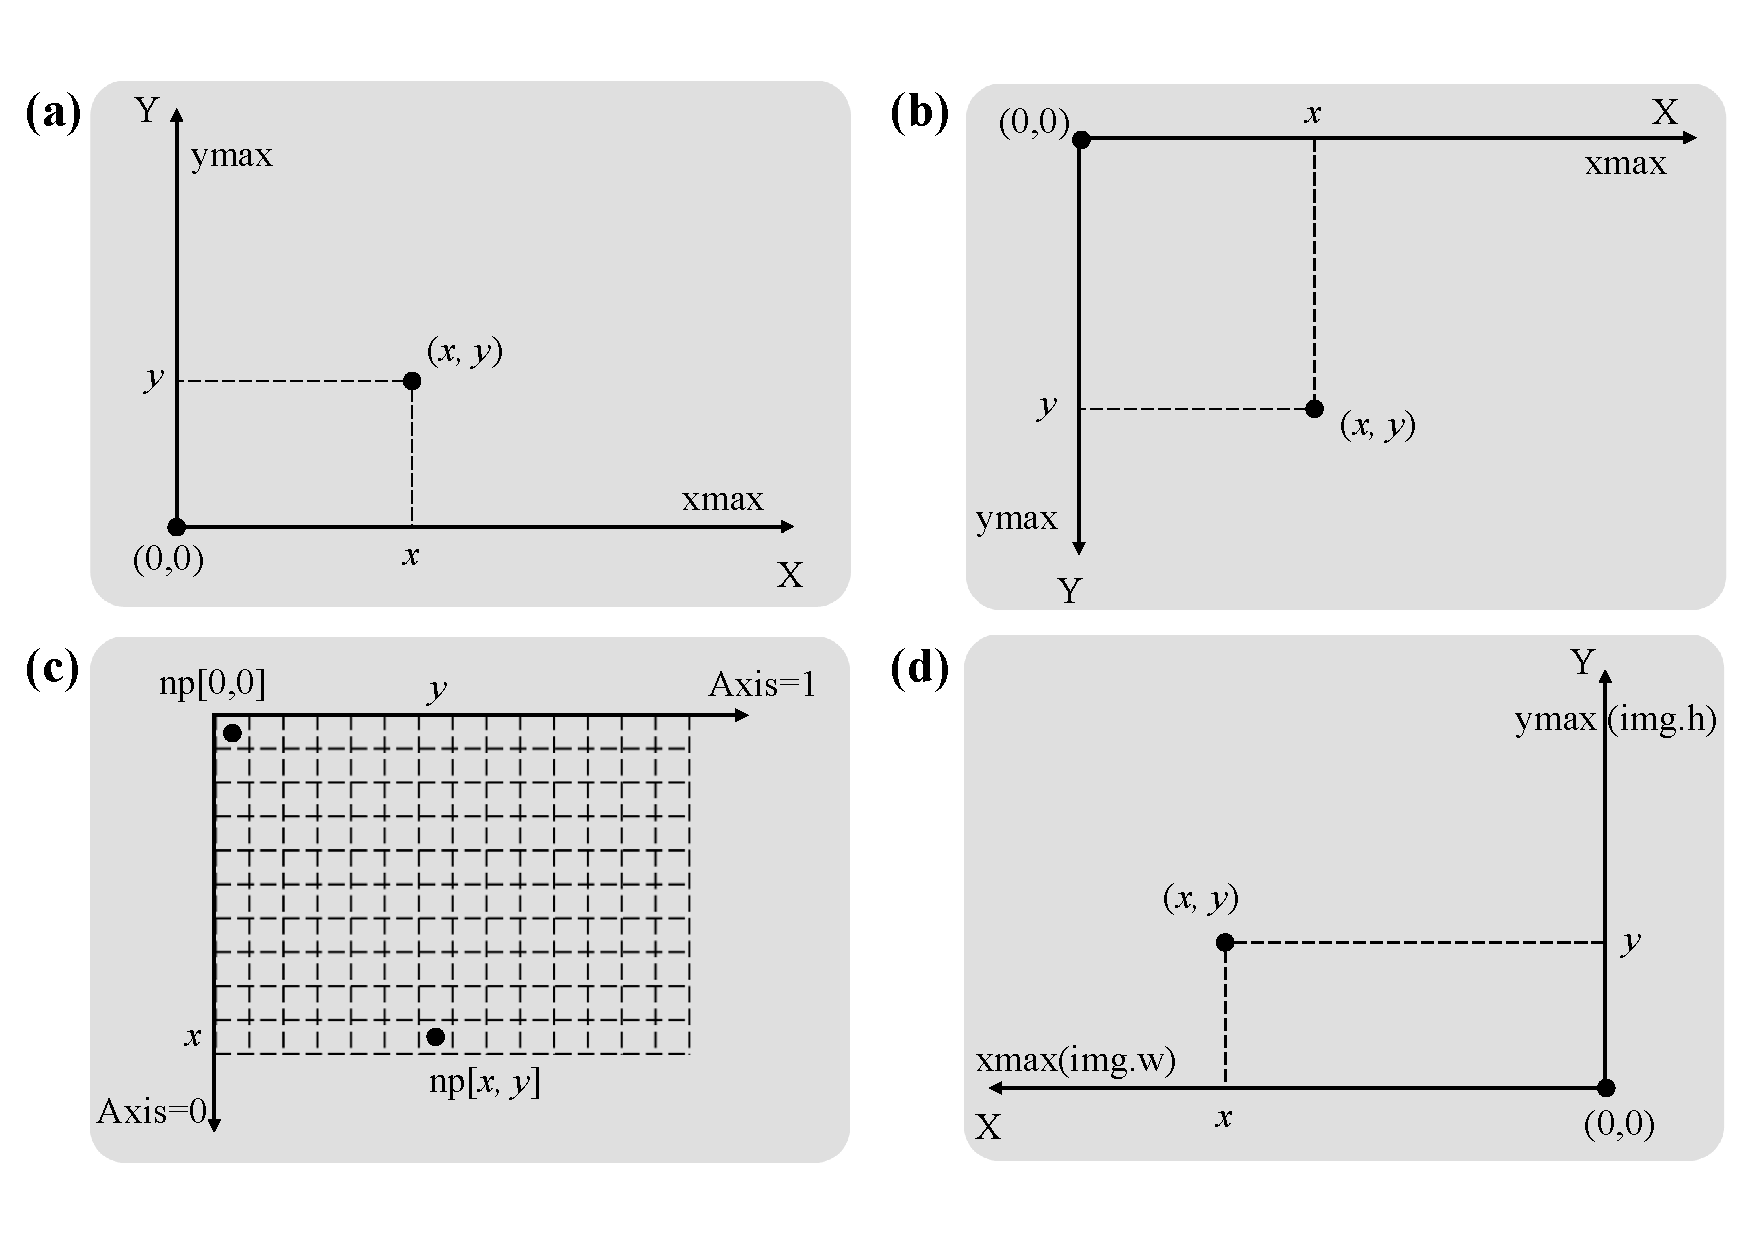
\includegraphics[width=0.95\linewidth]{figures/coordinates.pdf}
\caption{\csentence{The coordinates used}
  This need to be modified later, add 3D into it}
\end{figure}

\subsection*{Conversion algorithms}
1) from 2D Photo pixel coordinate to 2D Geo coordinate (DOM DSM, via GeoTiff header info)

2) 2D Geo coordinate to 3D Geo coordinate (Point clouds) via DSM (know xy, search z from DSM)

3) 3D Geo coordinate projects to 2D pixel coordinate via camera parameters from SfM output

4) [Future work] 2D photo pixel to 3D Geo coordinate without GIS information, using Shi Yun's algorithm, (not sure mention in this part or future work part)

\subsection*{Software dependency}
Python packages, platforms (Windows for exe)

Pix4D OpenSFM, FieldReconst (http://cse.naro.affrc.go.jp/rsugiura/FieldReconst/) introduction

\subsection*{Hardware dependency}
"\textit{For reliable performance of the system, server specifications of 8 GB of RAM and a multicore CPU with at least 3 GHz are recommended. The web-application can be accessed by any connected smart device capable of
running standard web-browsers.}" (copied from another software paper, need modification)

\section*{Results and discussion}

\subsection*{Software workflow}
Show the workflow chart 

\begin{figure}[htbp]
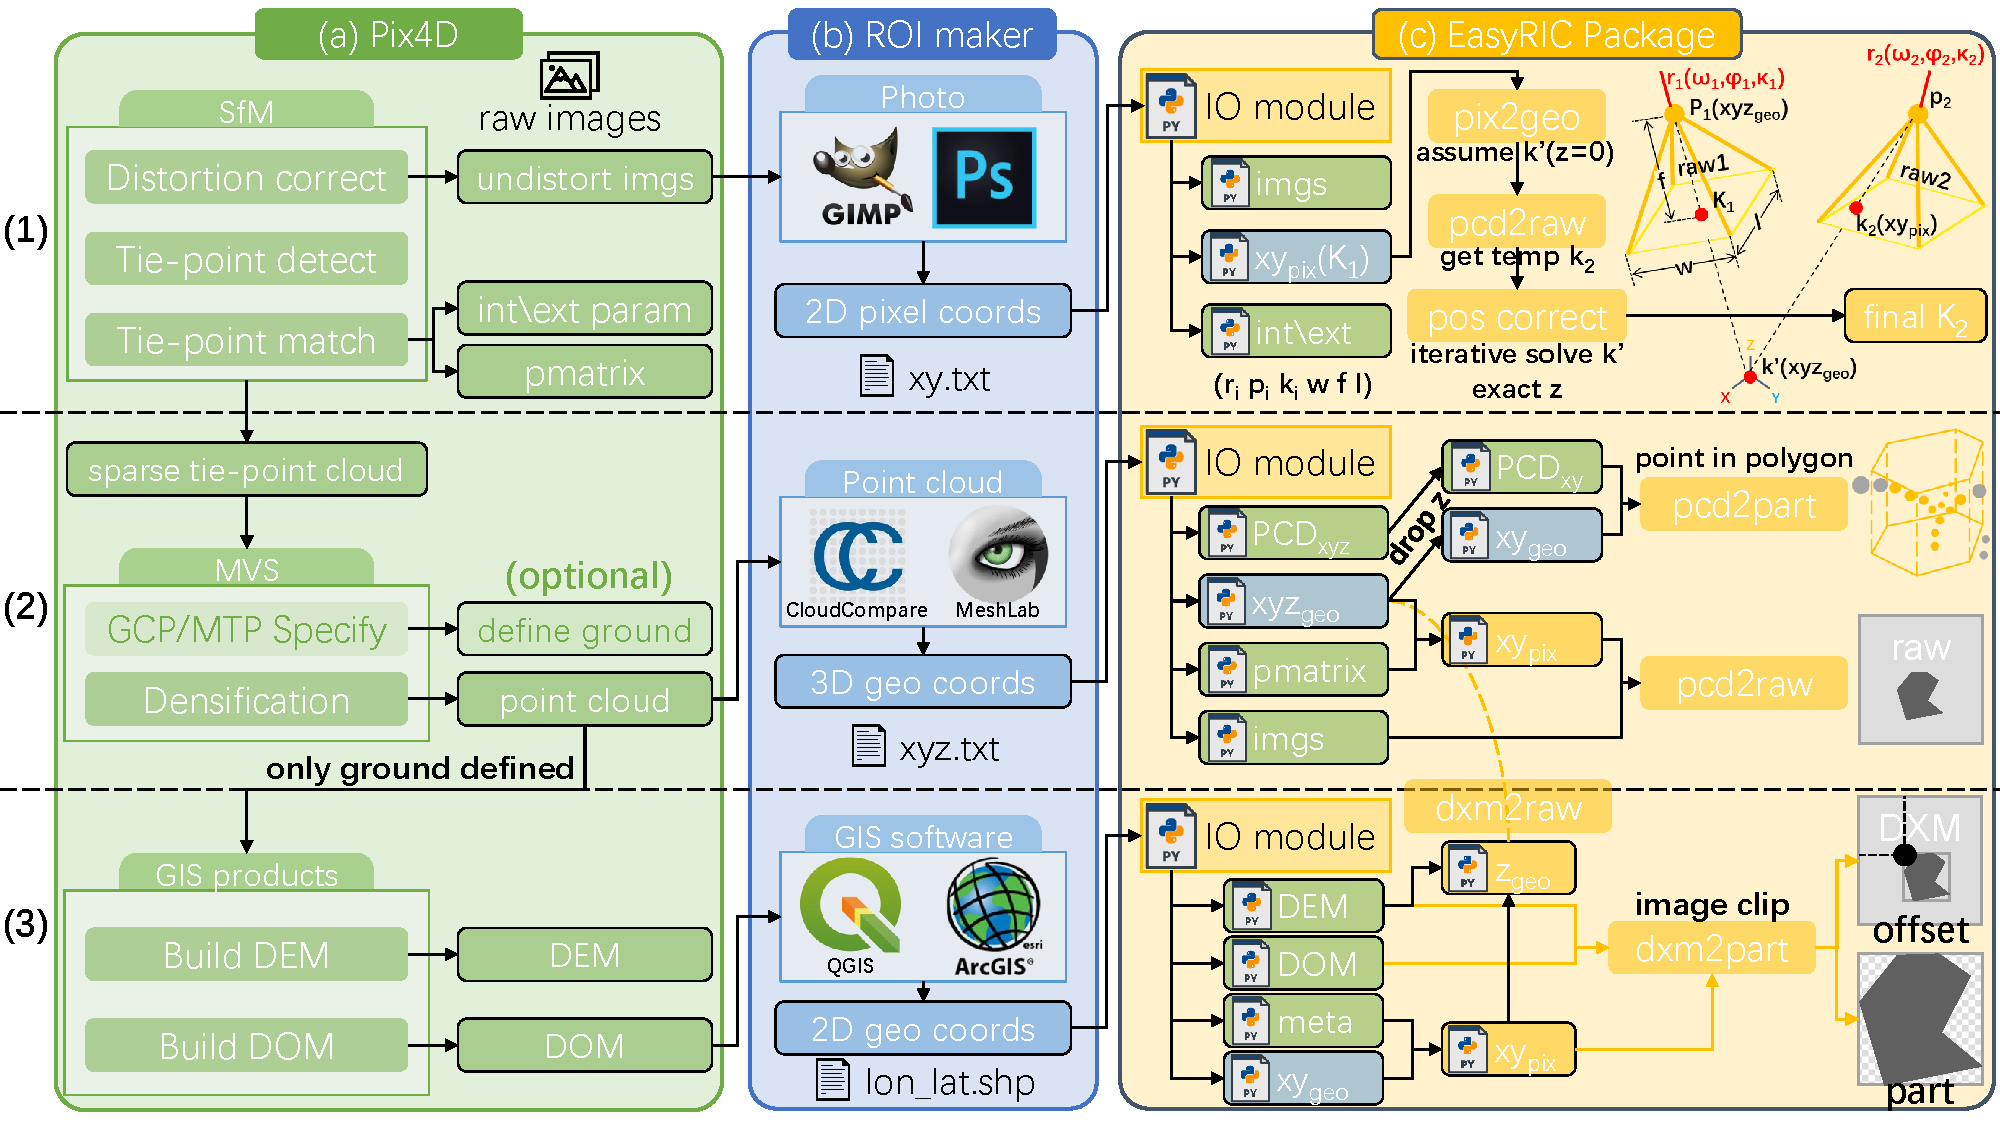
\includegraphics[width=0.95\linewidth]{figures/workflow.pdf}
\caption{\csentence{Workflow of software}
  This need to be modified later}
\end{figure}

\subsection*{Software operations}
Python command and classes to do previous workflow

Also introduce GUI interface (CMD line) if we have.

\subsection*{Package function analysis}

\subsubsection*{\acrshort{sfm} configuration}
It is quite important to ensure the quality of input data is analysiable. This part introduce the method about how to prepare raw images and \acrshort{sfm} outputs. 

Ground control points, flight speed etc.

\subsubsection*{Experimental design}
Experimental design about Lotus (Fig.  \ref{fig:plotid}), (in order to test this package, the following data were collected, and SfM products were produced by the following configs, using Pix4D as an exmaple)

\begin{figure}[htbp]
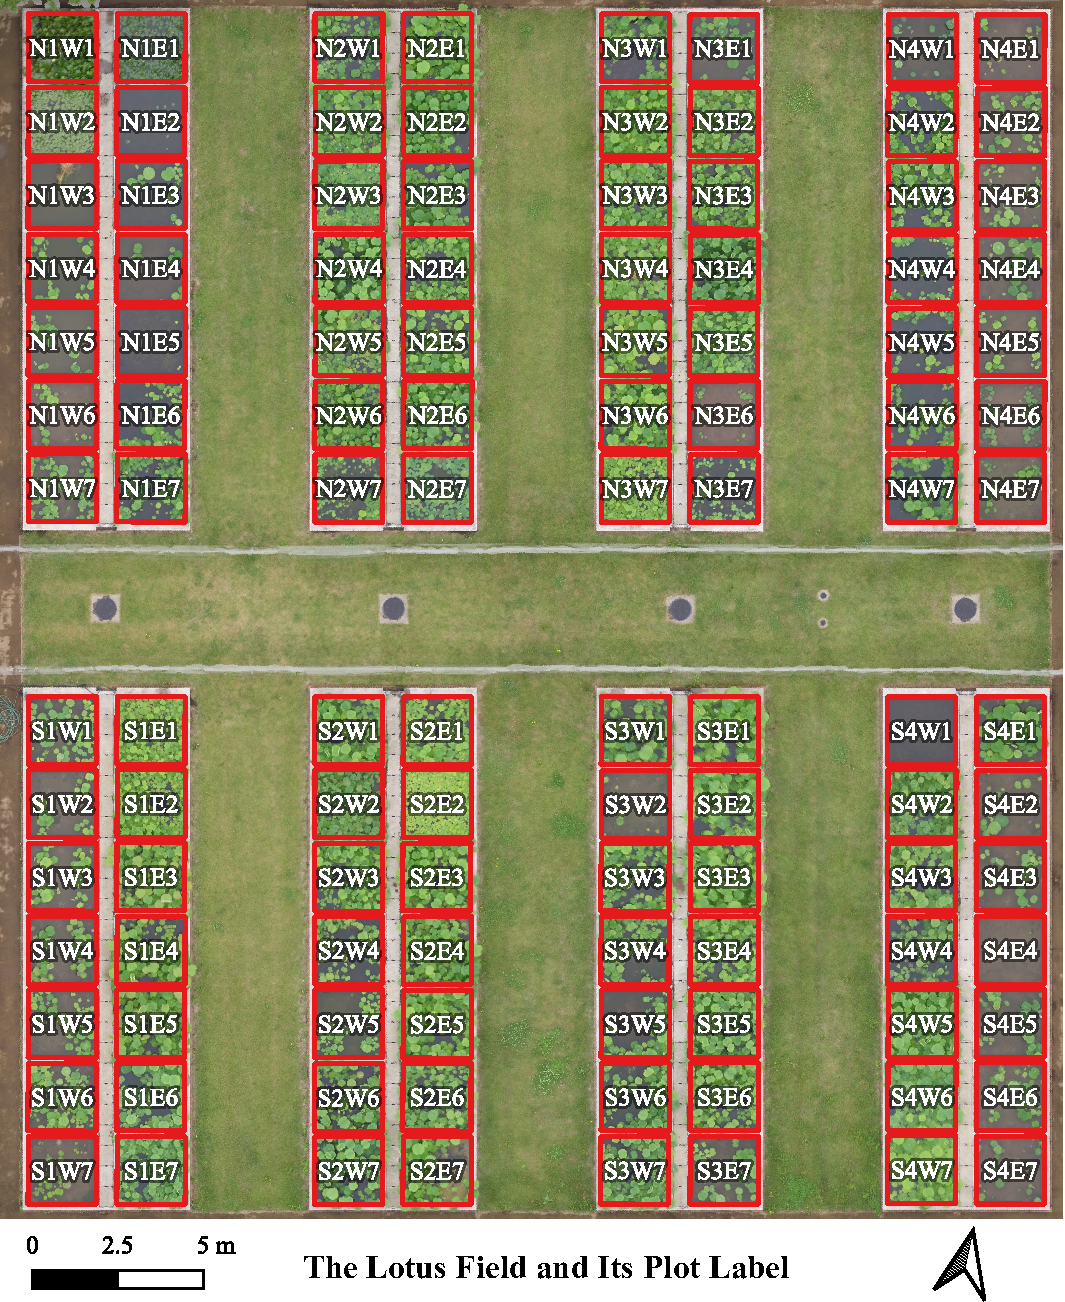
\includegraphics[width=0.95\linewidth]{figures/plot_with_id.pdf}
\caption{\csentence{Lotus plot id}localtion: Tokyo, Japan, DOM, 2017.05/09 made by QGIS, including this figure and label shapefile (shp), This need to be modified later}
\label{fig:plotid}
\end{figure}

\subsection*{Application examples}

\subsubsection*{Use case 1: Point cloud segmentation}
Compare \acrshort{roi} by time series

In this part, both raw photo? DOM? and point clouds should be displayed? Clipping point clouds may requires Open3D packages, which can not guarantee easy to be packed up.

\subsubsection*{Use case 2: plot segmentation}

Find \acrshort{roi} in \acrshort{sfm} products on the raw images

text \cite{ma_calculation_2019, guo_illumination_2013}
should including from DOM(DSM) coordinates (GIS or pixel) and point clouds (3D) coordinates to raw images.

\subsubsection*{Use case 3: Efficient annotation of training data for \acrshort{ml}/\acrshort{dl}}
3D/2.5D small region -> 2D->Raw small region, selecting strategy for efficient annotation of training data for ML/DL.

\subsection*{Future prospects}
API for most \acrshort{sfm} software packages

2D Photo to 2D photo without SfM products

Link between Aerial and Terristrial photos.

\section*{Conclusions}
Text

\section*{Availability and requirements}
\begin{itemize}
  \item \textbf{Project name:} EasyRIC
  \item \textbf{Project home page:} https://github.com/HowcanoeWang/EasyRIC
  \item \textbf{Operating system(s):} Using the source codes as Python package is platform independent, also providing executable software package for windows (windows 10 and 64-bit is tested and recommended).
  \item \textbf{Programming language: } Python
  \item \textbf{Other requirements:} For using source code as package: Python 3.7 or higher, numpy 1.18.1 or higher, scikit-image 0.16.2 or higher; For using executable software packages on Windows, 64-bit windows is required, and Intel CPU (with mkl support) is recommended.
  \item \textbf{License:} GPL-3.0
  \item \textbf{Any restrictions to use by non-academics:} Free to use for any purpose, forever.
\end{itemize}

\renewcommand*{\glsgroupskip}{}
\printglossary[type=\acronymtype, title=List of abbreviations]

%\paragraph*{Sub-sub-sub heading for section}
%Text for this sub-sub-sub-heading.

%%%%%%%%%%%%%%%%%%%%%%%%%%%%%%%%%%%%%%%%%%%%%%
%%                                          %%
%% Backmatter begins here                   %%
%%                                          %%
%%%%%%%%%%%%%%%%%%%%%%%%%%%%%%%%%%%%%%%%%%%%%%

\begin{backmatter}


\section*{Competing interests}
  The authors declare that they have no competing interests.

\section*{Author's contributions}
    Text for this section \ldots

\section*{Acknowledgements}
  Text for this section \ldots

%%%%%%%%%%%%%%%%%%%%%%%%%%%%%%%%%%%
%%                               %%
%% Additional Files              %%
%%                               %%
%%%%%%%%%%%%%%%%%%%%%%%%%%%%%%%%%%%

\section*{Additional Files}
  \subsection*{Additional file 1 --- Sample additional file title}
    Additional file descriptions text (including details of how to
    view the file, if it is in a non-standard format or the file extension).  This might
    refer to a multi-page table or a figure.

  \subsection*{Additional file 2 --- Sample additional file title}
    Additional file descriptions text.

\bibliographystyle{vancouver} % Style BST file (bmc-mathphys, vancouver, spbasic).
\bibliography{myzotero}

\end{backmatter}

\end{document}
